\section{The Cleaning Service}
\label{sec:cleaning}

This section presents the cleaning module, which enables users to identify quality problems in RDF data and to handle these problems either by removing all triples affected by problems (automatic cleaning using a web service) or in an interactive cleaning process using an OpenRefine extension for RDF cleaning. 

The great majority of details regarding functionality as well as the architecture of the cleaning module introduced in D3.1~\cite{d3.1} and D3.2~\cite{d3.2}, remains unchanged.
To keep this document short, we will not present them again. 
In this deliverable, we describe the changes and extensions that have been made in the resent period. 

The following improvements were made:
\begin{itemize}
\item Code reuse by integrating the cleaning web service into the OpenRefine extension
\item Implementation of a user friendly frontend interface for the cleaning web service
\item Automatic creation of an OpenRefine project from the given RDF data file
\item Extension of the cleaning report by statistics that summarise information about quality problems identified. Respectively, the QR Ontology introduced in D3.2~\cite{d3.2} has been extended by the corresponding terms. 
\end{itemize}
A detailed description of the particular changes as well as design decisions and implementation details will be presented in the corresponding subsections.

\subsection{Cleaning Workflow}
The Cleaning Module described in D3.2~\cite{d3.2} comprises two separate components – an OpenRefine\footnote{\url{http://openrefine.org/}} extension to clean data in interactive way, and the cleaning web service for automatical cleaning.
To offer the user a single entry point for both ways of cleaning, we have now integrated the web service into the OpenRefine extension without changing the functionalities of the single components.
The updated workflow of the cleaning process including both ways of cleaning is presented in Figure~\ref{fig:workflow}.

\begin{figure}[ht!]
\centering
% left bottom right top
\includegraphics[page=6,trim=0.5cm 4.5cm 2.5cm 0.5cm,clip,width=\textwidth]{figures/CleaningFigures.pdf}
\caption{Updated cleaning workflow}
\label{fig:workflow}
\end{figure}

The user starts cleaning by uploading his data and selecting the way he would like to clean data – interactive cleaning using OpenRefine or automatic cleaning by web services (Figure \ref{fig:entry}).
Several input data formats are supported\todo{CL: which ones?}.
By selecting “OpenRefine”, a corresponding OpenRefine project will be created from the defined data set, and the user will be forwarded to the OpenRefine perspective.
The web service provide two different cleaning methods: either the generation of cleaning suggestions, or deleting the problematic triples from the original data set.
More details about the different cleaning methods are presented in sections~\ref{sec:openrefine} and \ref{sec:cleaningService}.

\begin{figure}[ht!]
\centering
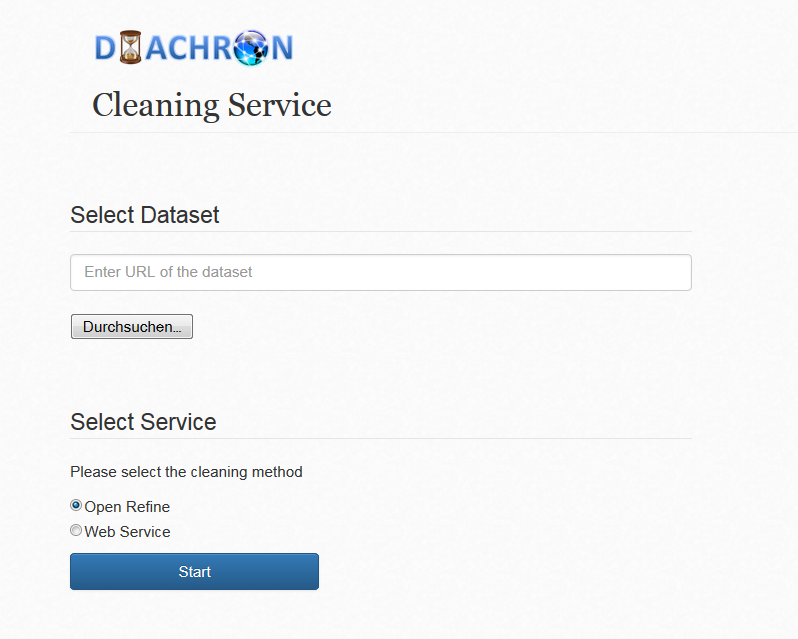
\includegraphics[width=11cm]{figures/CleaningStartPage.PNG}
\caption{User interface of Cleaning Module}
\label{fig:entry}
\end{figure}

\subsection{Cleaning with OpenRefine}
\label{sec:openrefine}

The mains steps of the cleaning workflow using OpenRefine, as initially described in D3.2~\cite{d3.2}, remain unchanged:
\begin{enumerate}
\item Creation of a project and representation of a data set as a “subject, predicate, object” table. In contrast to the previous cleaning module version, the backend automatically creates an OpenRefine project from the input file provided by the user. 
\item Identification of quality problems.  In this step the user defines a set of metrics according to his needs. The metric selection interface has slightly changed\todo{CL: in what way?}.  Figure~\ref{fig:metric_selection} shows the updated version.
\item Generation of cleaning suggestions and interactive cleaning.   To support the user in the cleaning process for the \textit{UndefinedClass} and \textit{UndefindedProperty} problems (i.e.\ using classes and properties for which no definition exists), we provide the user with concrete examples of classes or properties that could solve this problem. 
\todo{CL: please provide a short description of the used method, reference to used distance metric and a screenshot of the OpenRefine with this suggestion}
\item Export of cleaned data. The list of possible output formats has been extended to the most popular formats. The service now supports the \texttt{Turtle}, \texttt{RDF/XML}, \texttt{N-Triples}, and \texttt{N3} serialization formats.  We also implemented a user interface for this step (Figure~\ref{fig:export}).
\end{enumerate}




\begin{figure}[ht!]
\centering
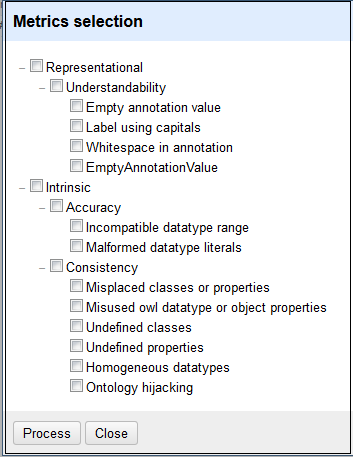
\includegraphics[width=6cm]{figures/MetricSelection.png}
\caption{Metric selection interface}
\label{fig:metric_selection}
\end{figure}



\begin{figure}[ht!]
\centering
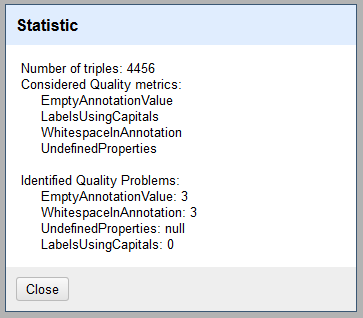
\includegraphics[width=8cm]{figures/statistics.png}
\caption{Cleaning statistics}
\label{fig:statistics}
\end{figure}


\begin{figure}[ht!]
\centering
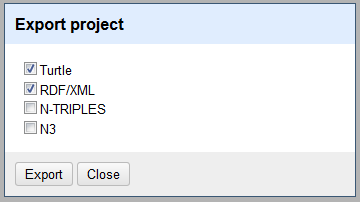
\includegraphics[width=6cm]{figures/export.png}
\caption{Export of cleaned data set in RDF format}
\label{fig:export}
\end{figure}

\subsection{Technical Documentation}


\subsubsection{Architecture design}
\todo{CL: UML diagram}
\subsubsection{Prerequisites}
\todo{CL: updated ontologies, new libraries}

\subsubsection{How to install}
To use the OpenRefine quality extension, you should follow one of the instruction lists given below.
\begin{description}
  \item[Build the extension from source code] \hfill \\
    The extension can be installed from scratch by building the OpenRefine project together with the quality extension.\\
    
  	Step 1. Check out the sources of OpenRefine from their GitHub repository.\\ 
    \textit{git clone https://github.com/OpenRefine/OpenRefine}\\
  
	Step 2. The extension must be checked out to the “extension” directory within the OpenRefine root directory.\\
	\textit{git clone https://github.com/diachron/quality-extension.git}\\
	
	Step 3. The two targets for cleaning and building the quality extension must be added to the ant build automation script (build.xml) in the “extension” directory of OpenRefine. The command \\ \textit{<ant dir="quality-extension/" target="build"/>} must be added to the \textit{build} target, and \\ \textit{<ant dir="quality-extension/" target="clean"/>} to the \textit{clean} target correspondingly.\\
	
	Step 4. The \textit{./refine build} command must be run to build the OpenRefine project together with the quality extension.
  
  \item[Install the extension with .zip file] \hfill \\
	The other way of installing the quality extension requires neither building the quality extension nor the OpenRefine project.  The installation follows a few simple steps:
	
	Step 1. Make sure that the OpenRefine project has already been installed on the local machine.\\
	
	Step 2. Run OpenRefine and browse to the “workspace” directory by clicking the link at the bottom of the project list.\\
	
	Step 3. Download the \textit{quality-extension.zip} file from the quality extension repository and extract into the “extension” directory in the workspace directory.\\
	
	Step 4. Restart OpenRefine.

\end{description}

\subsubsection{How to run}

OpenRefine with the installed extension can be run with the command \textit{./refine}.  This will start OpenRefine on \textit{localhost:3333}.
When a specific port and address is desired, use \textit{./refine -i 0.0.0.0 -p 3333}.

\subsubsection{Integration of new metrics}
The OpenRefine extension can easily be extended with new quality metrics.
To have a metric fully integrated into the extension, a developer would have to do the following steps.

\begin{itemize}
	\item A new metric class must be created in the \textit{com.google.refine.quality.metrics} package.  It must extend the abstract class \texttt{AbstractQualityMetric} by providing the implementation of its abstract methods.  The current implementation of this class provides minimal functionality – enough to use the metric within the extension. 
	
	Optionally, the metric can be enriched with a specific implementation of a related quality problem to end up in the cleaning report generated by the metric implementation.  This is achieved by extending the \texttt{QualityProblem} class located in the \textit{com.google.refine.quality.problems} package. The other improvement to the metric and quality problem pair would be enabling auto-cleaning functionality. It would take place after a simple implementation of the \texttt{AutoCleanable} interface, which has a single abstract method \textit{getCleanedStatement} with a return value of type \textit{Statement} (from the Jena RDF API).
	
	\item To enable the quality metric in the OpenRefine extension, it must be added to a JSON structure in the \textit{./module/scripts/metrics-dialog.js} JavaScript file in the form of a nested JSON data structure, for instance, \textit{\{"LabelsUsingCapitals" : "Label using capitals"\}}.  The key of this data structure must be the name of the metric class.
\end{itemize}

The above steps are sufficient to add a metric to the extension. When OpenRefine is running, an instance of the new metric class is created dynamically using using Java's reflection mechanism.  This new metric implementation approach that we are now employing facilitates the declaration of new metrics and improves the maintainability and readability of the code. 

%%% Local Variables: 
%%% mode: latex
%%% TeX-master: "D3.3"
%%% End: 
